%!TEX root = ../master.tex
\chapter{Development}\label{ch:development}
Our development chapter. \todo{We describe Rear Infused Illumination, and add all theory we have on the things mention if RID - for example BLOBs, contrast, illumination and so on }

\section{Rear Diffused Illumination}
The interaction on our game board table will be based on rear diffused illumination.\citep{multiTT} As shown in figure ((ref project sketch)) this means we are going to make inputs in the augmented board game via recognition of BLOBs shown in infra-red light, that are then observed by a camera beneath the table's surface. 
For this to work, a table's top surface made of transparent material needs a diffusermaterial just above or beneath it in order to diffuse the light. Infra-red light then needs to be shined on it from beneath the surface. When the glass is pressed from above the surface by an object, that part of the surface reflects more light back which will be captured by the camera as a BLOB.

\begin{figure}[!h]
\centering	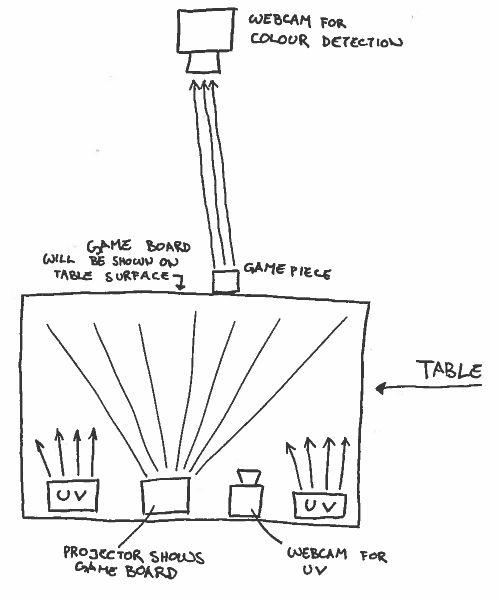
\includegraphics[width=0.5\textwidth]{TouchBoardDiagramSketch}
\end{figure}

Choosing such a solution has it's advantages and disadvantages. First of all, there is no need for a compliant surface or soldering for a LED frame, since we are using a diffuser in order to reflect the IR-light coming from below. The illuminators for that can be bought ready to go, so there is no need to build them. 

\section{Physical Design} 
This section will describe the physical aspect of our product.
We have assembled a touch board, made with a plexi glass top and IR lamps below. Underneath the top is a short throw projector so we are able to project images on the top. Additionally we have a web camera on the very bottom of the table to be able to detect, via the IR lamps any changes, in form of touches or placed game pieces, in the surface of the board. 
The field of view of the camera is 74cm*58cm, and the entire table top is 102cm*120cm. The table is 95cm. 
a

\section{Technology}

